\documentclass[
    12pt, % Schriftgröße
    oneside, % zweiseitiger Modus
    ngerman, % deutsches Dokument
    BCOR=0mm, % Bindungskorrektur
    DIV=10 % Division (Anzahl Spalten/Zeilen pro Seite, bestimmt implizit Margins)
]{scrreprt}

\newcommand{\titleDocument}{Abgabeübung COBOL Dreiecksberechnung}
\newcommand{\authorDocument}{Leon Jarosch}
\newcommand{\subjectDocument}{Abgabeübung}
\newcommand{\locationDocument}{Köln}
\newcommand{\dateDocument}{\today} % Alternativ z.B. 30.~September 2021

\title{\titleDocument}
\author{\authorDocument}
\date{\dateDocument}

\usepackage{dokumentation}

\begin{document}
    % ============ Anfang =============
    % Titelseite
    \begin{titlepage}
	% TODO: wird das geometry Paket genutzt statt der Mechanismen aus KOMA-Skript, kann die folgende Zeile z.B. durch "\newgeometry{...}" ersetzt werden
	\typearea{100} % DVI auf 100 setzen für Titel (kleine Margins)
	\setlength{\parindent}{0pt} % keine Einrückung bei neuen Absätzen auf dieser Seite

	\begin{flushright}
		
\includegraphics[height=5cm]{images/FH-Aachen-r_svg-raw}
	\end{flushright}
	
	\vspace*{-2.5cm}

	\begin{center}
		\textbf{\Huge Fachhochschule~Aachen}

		\vspace*{0.5cm}
		
		\textbf{\Huge Studienort Köln}

		\vspace*{0.75cm}

		{\normalsize\doublespacing Fachbereich~9:~Medizintechnik~und~Technomathematik\\	Studiengang:~Angewandte~Mathematik~und~Informatik}

		\vspace*{2.5cm} % TODO: bei mehr verwendeten Zeilen für den Titel verringern
		
		\begin{minipage}[t]{14cm} % TODO: abhängig von dem konkreten Titel muss diese Breite eventuell angepasst werden für einen passenden Zeilenumbruch
			\begin{center}
				\textbf{\Huge \titleDocument}
			\end{center}
		\end{minipage}
	
		\vspace*{2.5cm} % TODO: bei mehr verwendeten Zeilen für den Titel verringern (symmetrisch zu oben)
		
		\textbf{\Large \subjectDocument}

		\vspace*{0.5cm}
		
		{\normalsize von}
		
		\vspace*{0.5cm}
		
		\textbf{\Large \authorDocument}
	
		\vspace*{3.5cm}
		
		\begin{minipage}[t]{13cm}
			\begin{center}
				\begin{tabular}{llll}
					Matrikelnummern: & 3237534 & 3240219 & 3235914 \\
				\end{tabular}
			\end{center}
		\end{minipage}
		
		\vspace*{2.5cm}
	
		{\large \locationDocument, den \dateDocument}
	\end{center}
\end{titlepage}


    % Eidesstattliche Erklärung und Abstrakt
%    \begingroup
    % keine Seitenzahl und kein running header
%    \thispagestyle{empty}
%    \renewcommand*{\chapterpagestyle}{empty}

%    \cleardoubleoddpage % Abstrakt rechts

%    \glsresetall % alle bereits genutzten Akronyme wieder zurücksetzen
%    \endgroup

    % Inhaltsverzeichnis
%    \cleardoubleoddpage % Inhaltsverzeichnis rechts
%    \thispagestyle{plain}
    \tableofcontents

    % =========== Zahlenteil ===========
    \chapter{Programmbeschreibung}\label{ch:programmbeschreibung}

\section{Programmablaufplan}\label{sec:pap}
Der Ablauf des Programms ist sequenziell und kann daher gut mit Programmablaufplänen dargestellt werden.
Die folgenden Abbildungen beschreiben Teile des Programms.
Abbildung~\ref{fig:diagramm1} zeigt, wie aus wiederholten Benutzereingaben Sätze konstruiert werden.
Die Auswahl eines externen Wörterbuchs wird in Abbildung ~\ref{fig:diagramm2} beschrieben.
In Abbildung~\ref{fig:diagramm3} wird der Ablauf des Explizimodus visualisiert.
Die Ermittlung eines Wortes, aus einem eingegebenen T9-Code, kann in Abbildung~\ref{fig:diagramm4} beobachtet werden.


% \begin{figure}[!h]
%     \centering
%     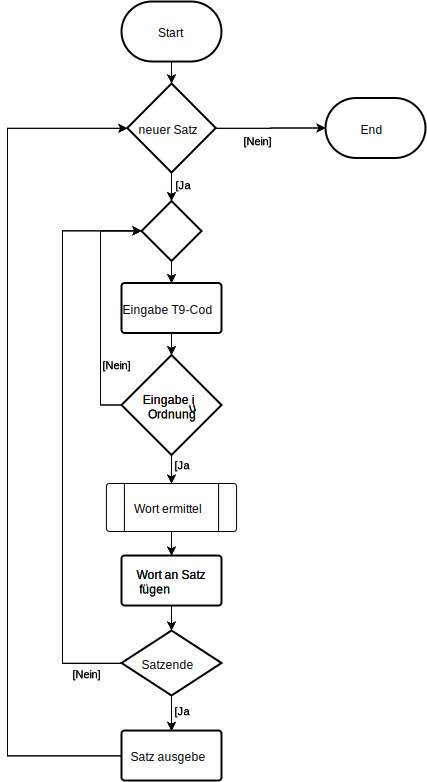
\includegraphics[scale=0.9,width=\textwidth,height=\textheight,keepaspectratio]{Benutzerdialog}
%     \caption{
%         Benutzerdialog: Konstruieren von Sätzen aus Sicht des Anwenders.
% %        Zunächst werden Wörter eingelesen, falls der Satz beendet wird, wird er ausgegeben.
% %        Das Programm wird beendet, falls der finale Satz leer ist und ein Punkt eingegeben wird.
%     }
%     \label{fig:diagramm1}
% \end{figure}

% \begin{figure}[!h]
%     \centering
%     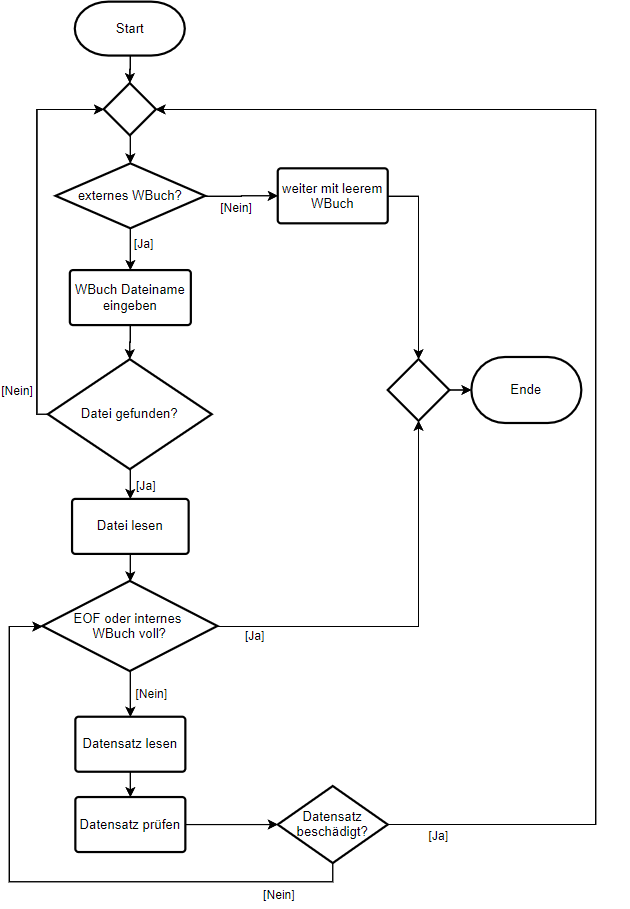
\includegraphics[width=\textwidth,height=\textheight,keepaspectratio]{Einlesen_WBuch1}
%     \caption{
%         Einlesen eines externen Wörterbuchs.
% %        Der Benutzer wird gefragt, ob ein externes Wörterbuch eingelesen werden soll.
% %        Der Benutzer möchte ein externes Wörterbuch einlesen, dann wird jeder Datensatz gelesen, geprüft und in das interne Wörterbuch gespeichert, wenn die Prüfung des Datensatzes erfolgreich war.
% %        Das Einlesen wird abgebrochen, sobald ein Fehler in der Prüfung ist.
% %        Falls die einzulesende Datei nicht gefunden wird, fängt die Methode von vorne an.
% %        Wenn der Benutzer kein externes Wörterbuch nutzen möchte, wird ein neues erstellt.
%     }
%     \label{fig:diagramm2}
% \end{figure}

% \begin{figure}[!h]
%     \centering
%     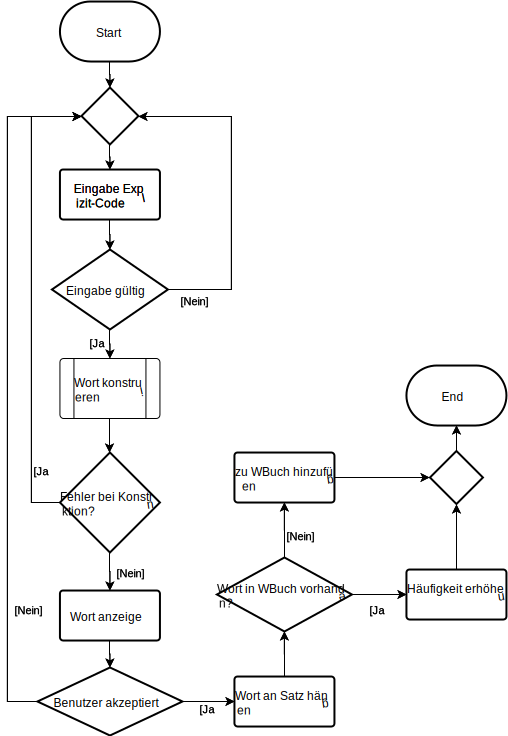
\includegraphics[width=\textwidth,height=\textheight,keepaspectratio]{Explizitmodus}
%     \caption{
%         Ablauf des Explizitmodus.
% %        Zunächst gibt der Benutzer ein Wort in expliziter Darstellung ein.
% %        Dieses wird geprüft und danach konstruiert.
% %        Der Benutzer prüft das konstruierte Wort, falls das Wort dem Wunsch des Benutzers entspricht, wird noch geschaut, ob es im Wörterbuch bereits vorhanden ist.
% %        Wenn es schon vorhanden war, wird die Häufigkeit erhöht, sonst wird das neue Wort mit dem zugehörigen Code und der Häufigkeit eins dem Wörterbuch hinzugefügt.
%     }
%     \label{fig:diagramm3}
% \end{figure}

% \begin{figure}[!h]
%     % \centering
%     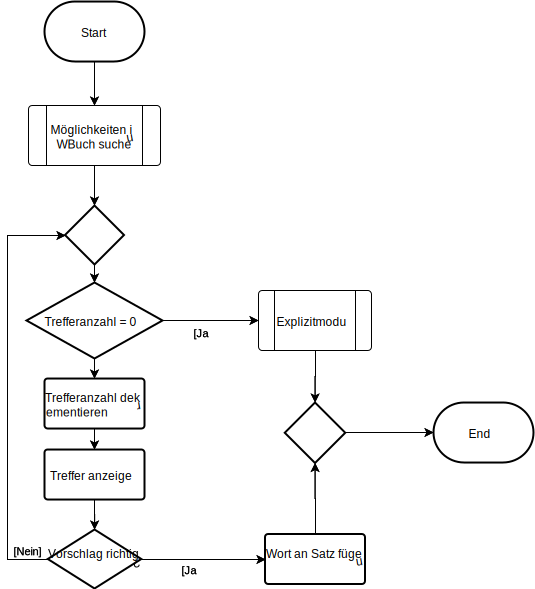
\includegraphics[width=\textwidth,height=\textheight,keepaspectratio]{Wort_ermitteln}
%     \caption{
%         Ermitteln eines Wortes.
% %        Wort ermitteln: Zu Beginn wird im Wörterbuch geschaut, ob der eingegebene Code vorhanden ist.
% %        Die Treffer werden dem Benutzer nacheinander angezeigt, je nach der Benutzerrückmeldung wird der nächste Vorschlag angezeigt oder an den Satz angefügt.
% %        Falls die Trefferanzahl gleich null ist, wird der Benutzer in den Explizitmodus weitergeleitet.
%     }
%     \label{fig:diagramm4}
% \end{figure}


\section{Entwicklungsdokumentation}\label{sec:entwicklerdokumentation}


Es wurden grundsätzlich sprechende Namen für Variablen, Abschnitte und Paragrafen gewählt.
Daher bedarf es nur geringer Dokumentation.
Die Funktionen der einzelnen Paragrafen sind in Tabelle~\ref{tab:prog-strukt} beschrieben.

Wenn Variablen zu einer bestimmten logischen Einheit gehören, haben sie einen passenden Präfix.

\definecolor{fhfarbe}{HTML}{51B2AC}
\definecolor{fhfarbe2}{HTML}{4FAEAB}
\begin{table}[!htb]
    \centering
    \rowcolors{2}{black!5}{white}
    \begin{tabularx}{\textwidth}{X | X }
       \rowcolor{fhfarbe!25}
       Bezeichnung                             & Beschreibung             \\
%       \hline
       MAIN-PROCEDURE & Hauptablauf, in dem einzelne Aufgaben an andere Paragrafen delegiert werden \\
       \rowcolor{fhfarbe!10}
       Vorlauf SECTION & Abschnitt zur Vorbereitung des Programms  \\
       Auswahl-WBuch & Es wird die Auswahl eines externen Wörterbuchs angeboten  \\
       Einlesen-WBuch & Paragraf zum Einlesen eines, zuvor spezifizierten, Wörterbuchs  \\
       Lese-Satz & Verarbeitungsschritt einer einzelnen Zeile eines externen Wörterbuchs   \\
       Init-Explizit-Tab & Initialisierung des strukturellen Aufbaus der Handytastatur  \\
       \rowcolor{fhfarbe!10}
       Hauptlauf SECTION & Abschnitt zur Hauptaufgabe des Programms  \\
       Benutzer-Dialog & Paragraf zum Steuern des Benutzer-Dialogs \\
       Ermittle-Wort & Ermittelt ein Wort aus einem eingegebenen T9-Code  \\
       Wort-Auswahl &  Paragraf schlägt passende Wörter zum eingegebenen T9-Code vor, und ermöglicht eine Auswahl \\
       Finde-Moeglichkeiten & Es werden alle, zum eingegebenen Code passenden, Wörter im Wörterbuch gefunden und zwischengespeichert   \\
       Sortiere-Nach-Haeuf & Bubble-Sort zum Sortieren der zwischengespeicherten Treffer  \\
       Explizit-Eingabe & Steuerung der Eingabe im Explizitmodus  \\
       Suche-Wort-In-WBuch & Prüft, ob ein Wort bereits im Wörterbuch vorhanden ist  \\
       Konstruiere-Wort & Konstruiert ein Wort aus einem eingegebenen Explizit-Code  \\
       Pruefe-Explizit-Eingabe &  Validiert eine Benutzereingabe im Explizitmodus \\
       Pruefe-Eingabe & Validiert eine Benutzereingabe im normalen Modus \\
       \rowcolor{fhfarbe!10}
       Nachlauf SECTION & Abschnitt zum Speichern des Wörterbuchs \\
       Schreibe-WBuch-Sortiert &  Sortiert das Wörterbuch alphabetisch und speichert es in einer Datei \\
    \end{tabularx}
    \caption{Aufgaben der einzelnen logischen Einheiten.}\label{tab:prog-strukt}
\end{table}

    \chapter{Verfahrensbeschreibung}\label{ch:verfahrensbeschreibung}


\section{Mathematischer Hintergrund}\label{sec:mathematischer_hintergrund}
Das System arbeitet verschiedenen mathematischen Verfahren mit welchen die benötigten Berechnungen durchgeführt werden.

\subsection{Formel von Heron}\label{subsec:formel_von_heron}
Zum berechnen des Flächeninhalts eines Dreiecks wird die Formel von Heron verwendet.
\\
Der Satz von Heron besagt, dass die Fläche eines Dreiecks durch die Länge seiner Seiten berechnet werden kann. Mathematisch ausgedrückt:

\begin{align}
    A=\sqrt{s(s-a)(s-b)(s-c)}\\
\end{align}
Wobei $s$ für die Hälfte des Umfangs steht:
\begin{align}
    s=\frac{a+b+c}{2}
\end{align}

\subsection{Satz des Pythagoras}\label{subsec:satz_des_pythagoras}
Zum überprüfen ob ein Dreieck rechtwinklig ist, wird der Satz des Pythagoras verwendet.
\\
Der Satz des Pythagoras besagt, dass in einem rechtwinkligen Dreieck die Summe der Kathetenquadrate gleich dem Hypothenusenquadrat ist. Mathematisch ausgedrückt:

\begin{align}
    a^2+b^2=c^2\\
\end{align}

Bildlich veranschaut sieht die Formel wie folgt aus:

\begin{figure}
    \centering
    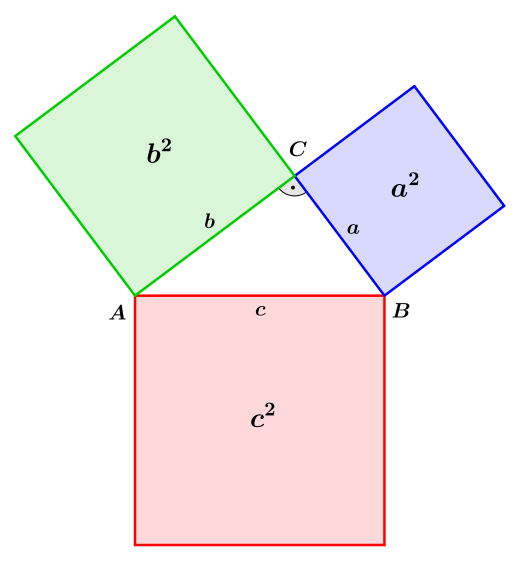
\includegraphics[width=0.5\textwidth]{images/pythagoras.png}
    \caption{Satz des Pythagoras}
    \label{fig:pythagoras}
\end{figure}

    \chapter{Testdokumentation}\label{ch:testdokumentation}
Im folgenden Testfälle mit welchem das Programm getestet wurde.

\definecolor{fhfarbe}{HTML}{00605E}


\section{Vordefinierte Tests}\label{sec:definierte_tests}


% \begin{tabular}{|c|c|c|c|c|c|}
%     \hline
%     a & b & c & U & F & Art \\
%     \hline
%     5 & 3 & 4 & 12 & 6,00 & r, s \\
%     \hline
%     11 & 11 & 10 & 32 & 48,990 & nr, gsch \\
%     \hline
%     29 & 29 & 29 & 87 & 364,164 & nr, gs \\

%     \hline
% \end{tabular}

\begin{figure}
    \centering
    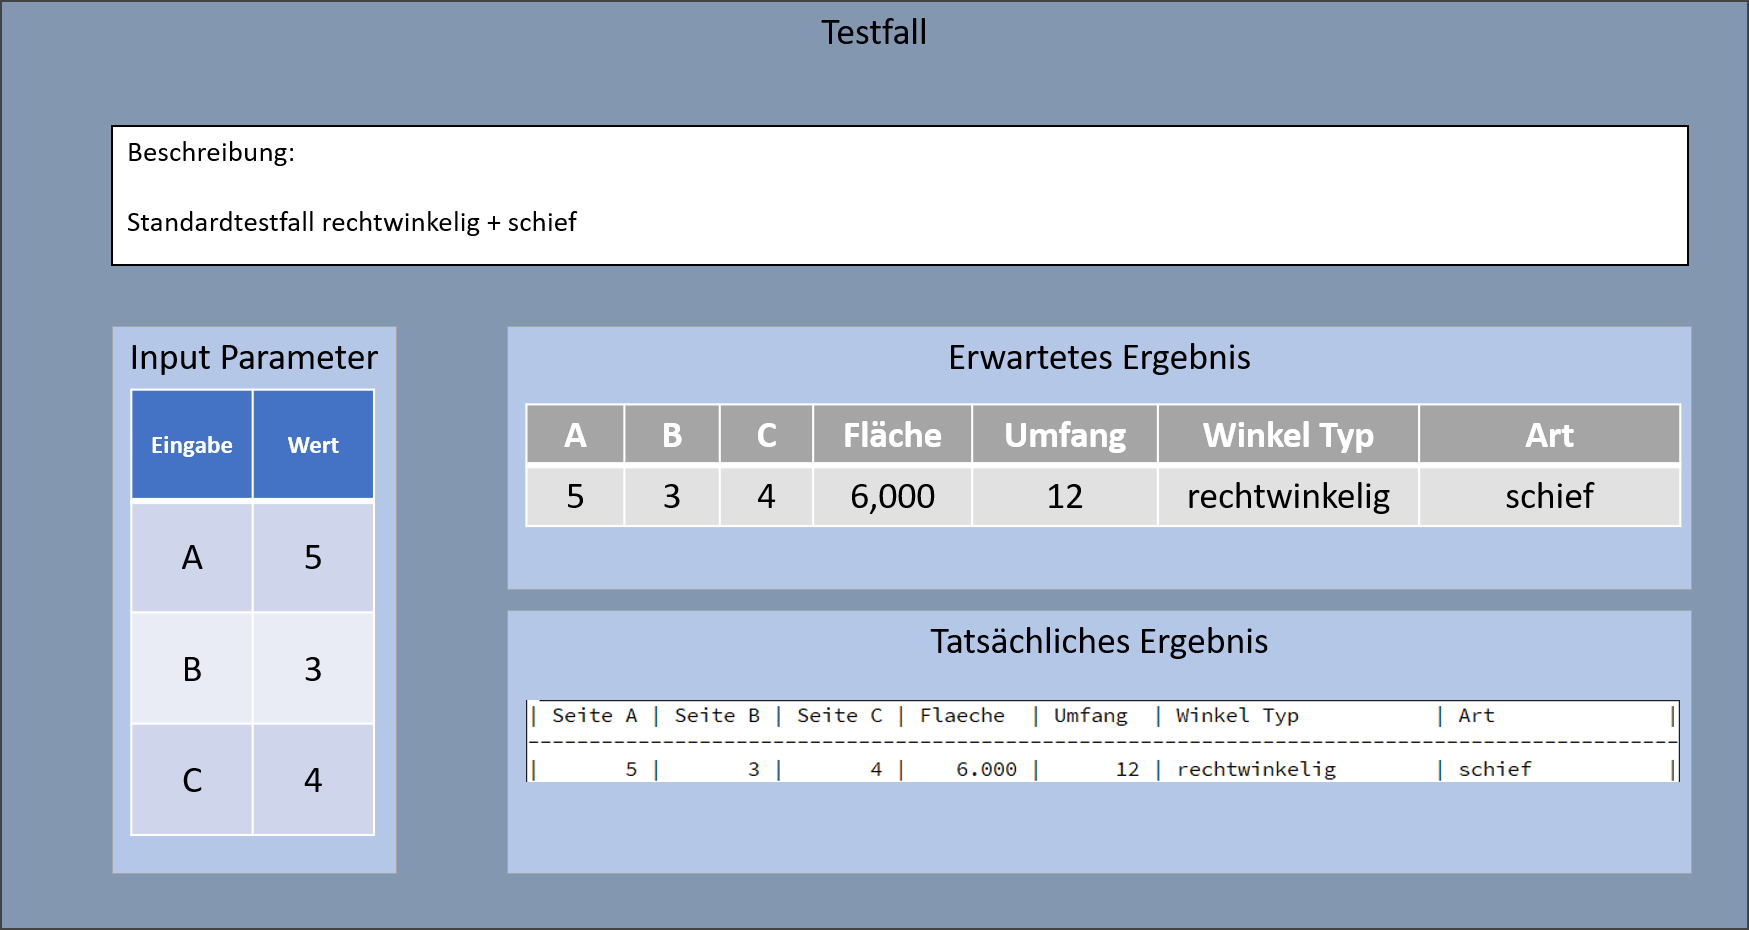
\includegraphics[width=\linewidth]{images/Testfall1.png}
    \caption{Testfall 1}
\end{figure}

\begin{figure}
    \centering
    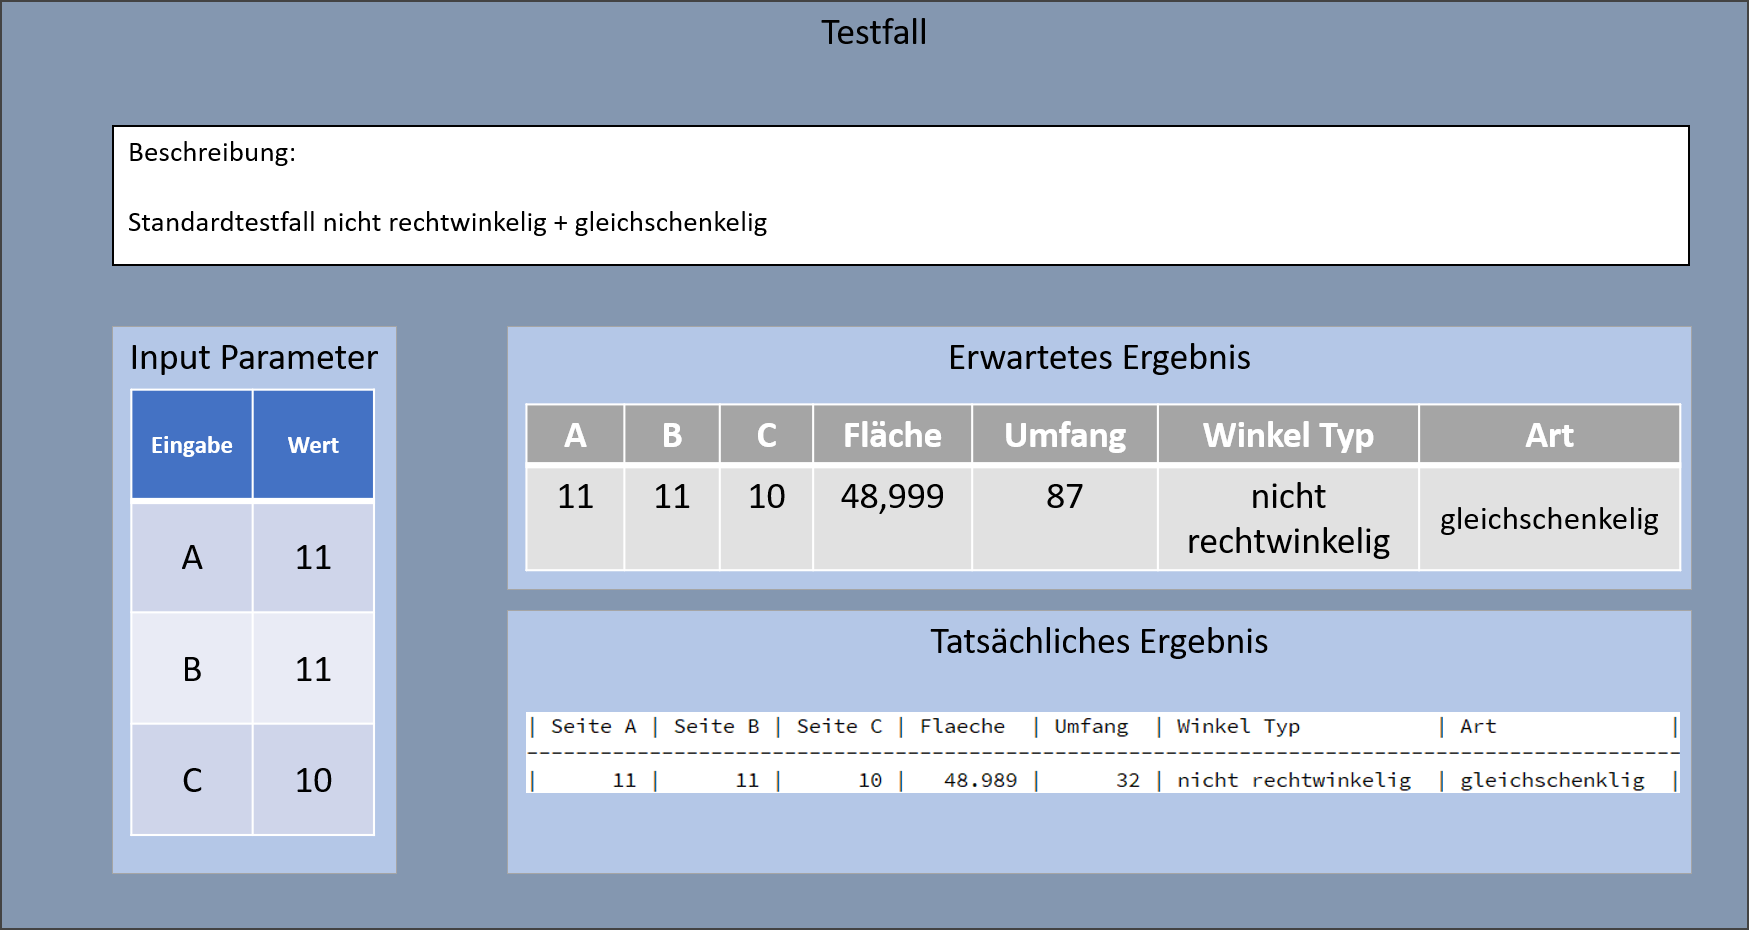
\includegraphics[width=\linewidth]{images/Testfall2.png}
    \caption{Testfall 2}
\end{figure}

\begin{figure}
    \centering
    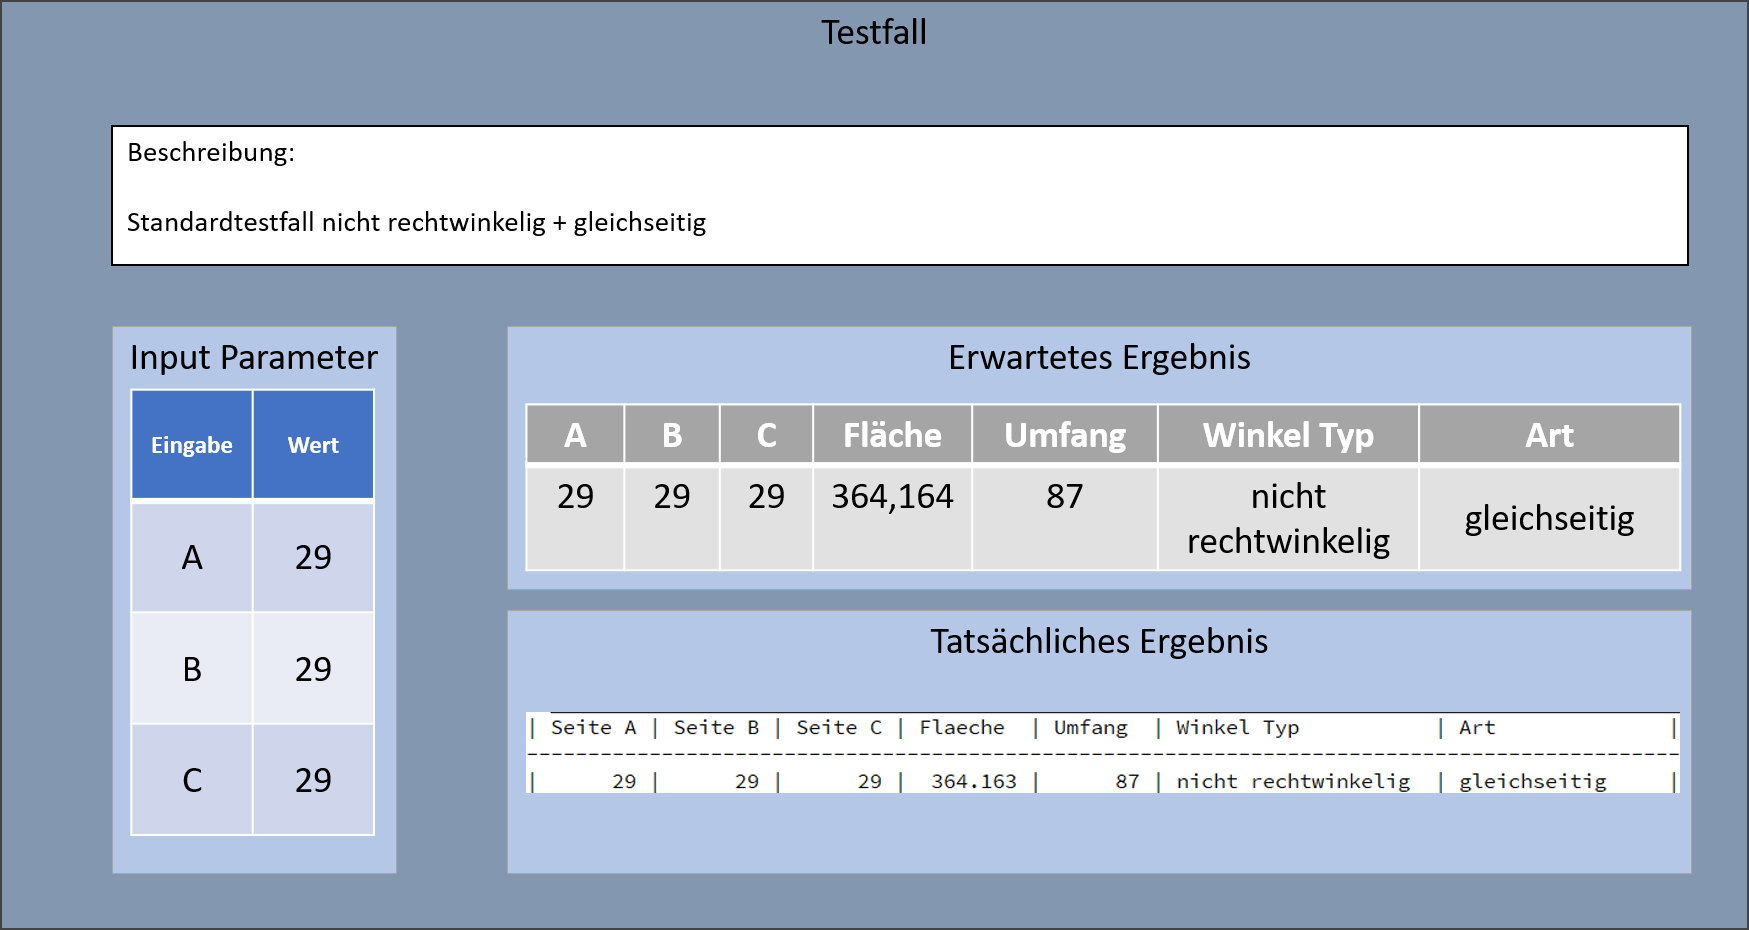
\includegraphics[width=\linewidth]{images/Testfall3.png}
    \caption{Testfall 3}
\end{figure}

\section{Ergänzende Tests}\label{sec:ergänzende_tests}

\begin{figure}
    \centering
    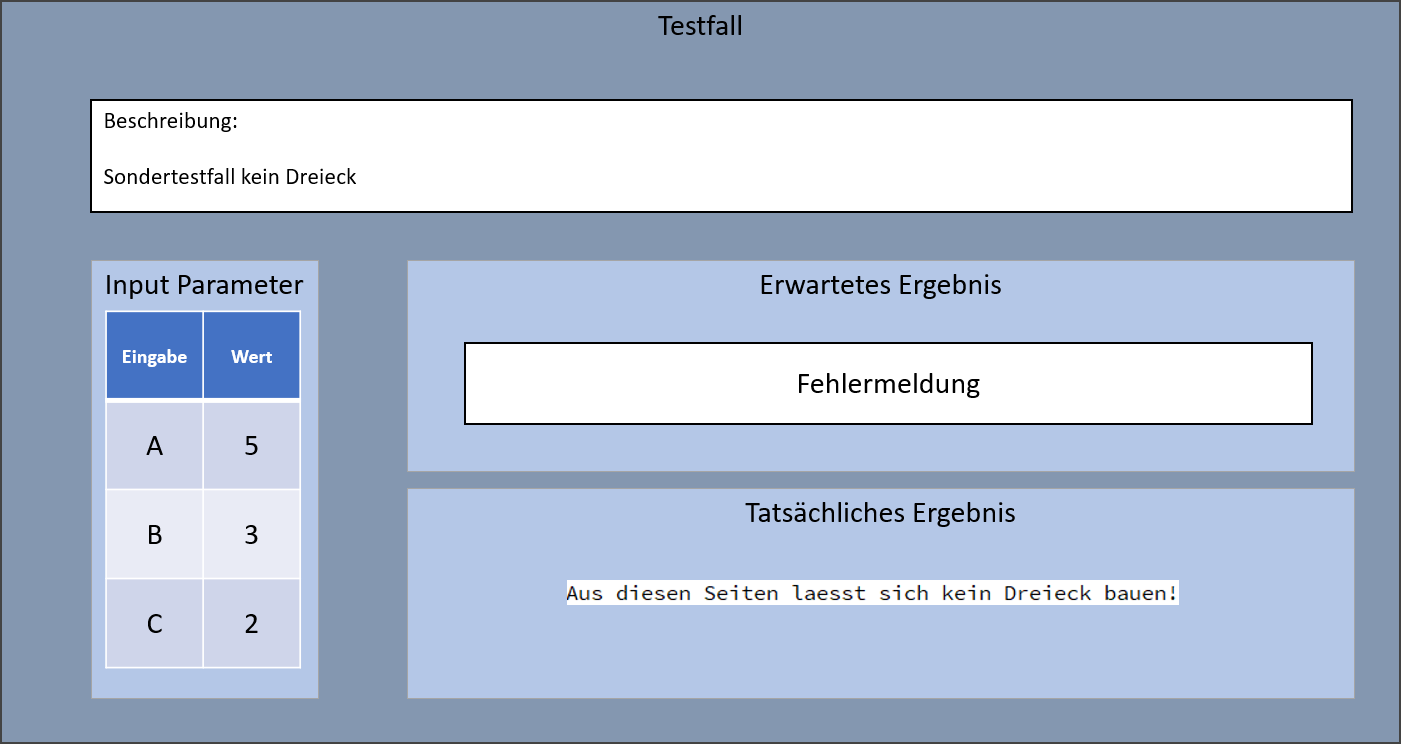
\includegraphics[width=\linewidth]{images/Testfall4.png}
    \caption{Testfall 4}
\end{figure}

\begin{figure}
    \centering
    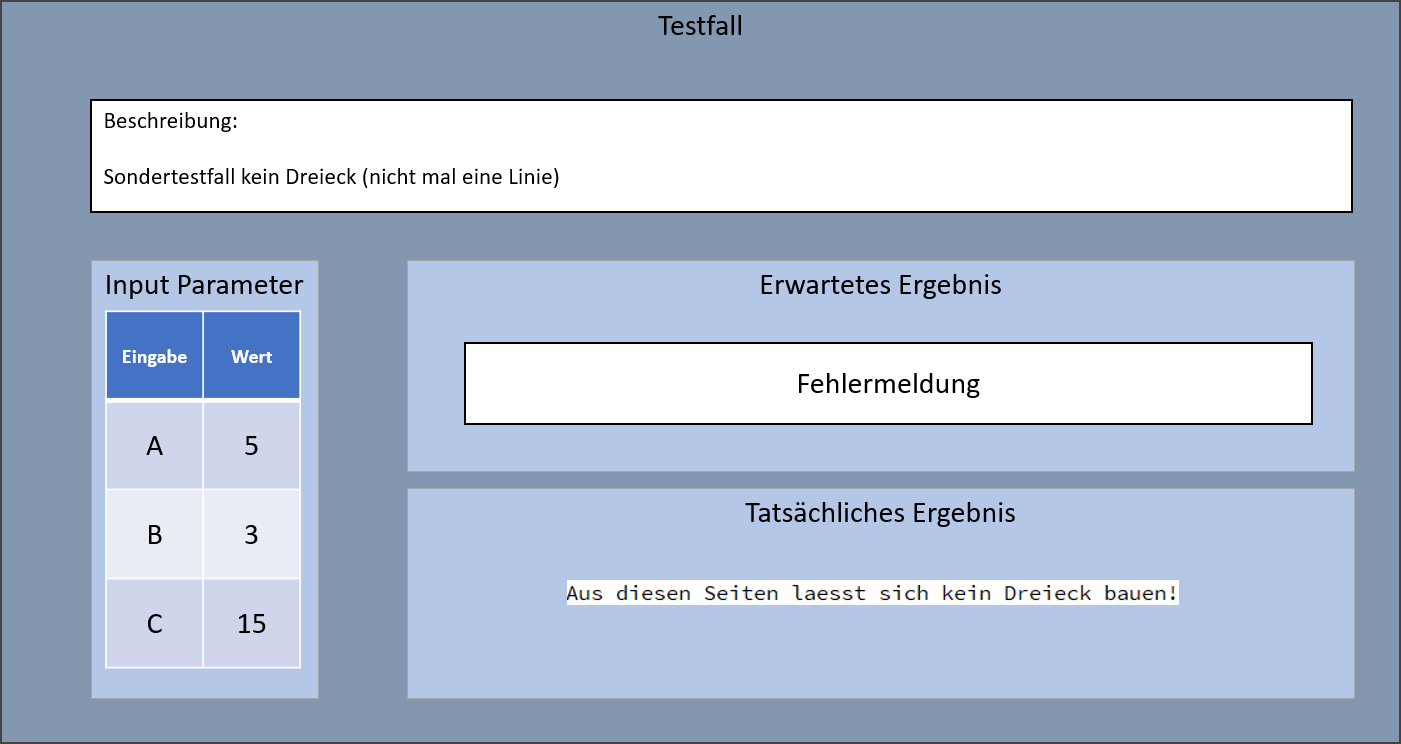
\includegraphics[width=\linewidth]{images/Testfall5.png}
    \caption{Testfall 5}
\end{figure}

\begin{figure}
    \centering
    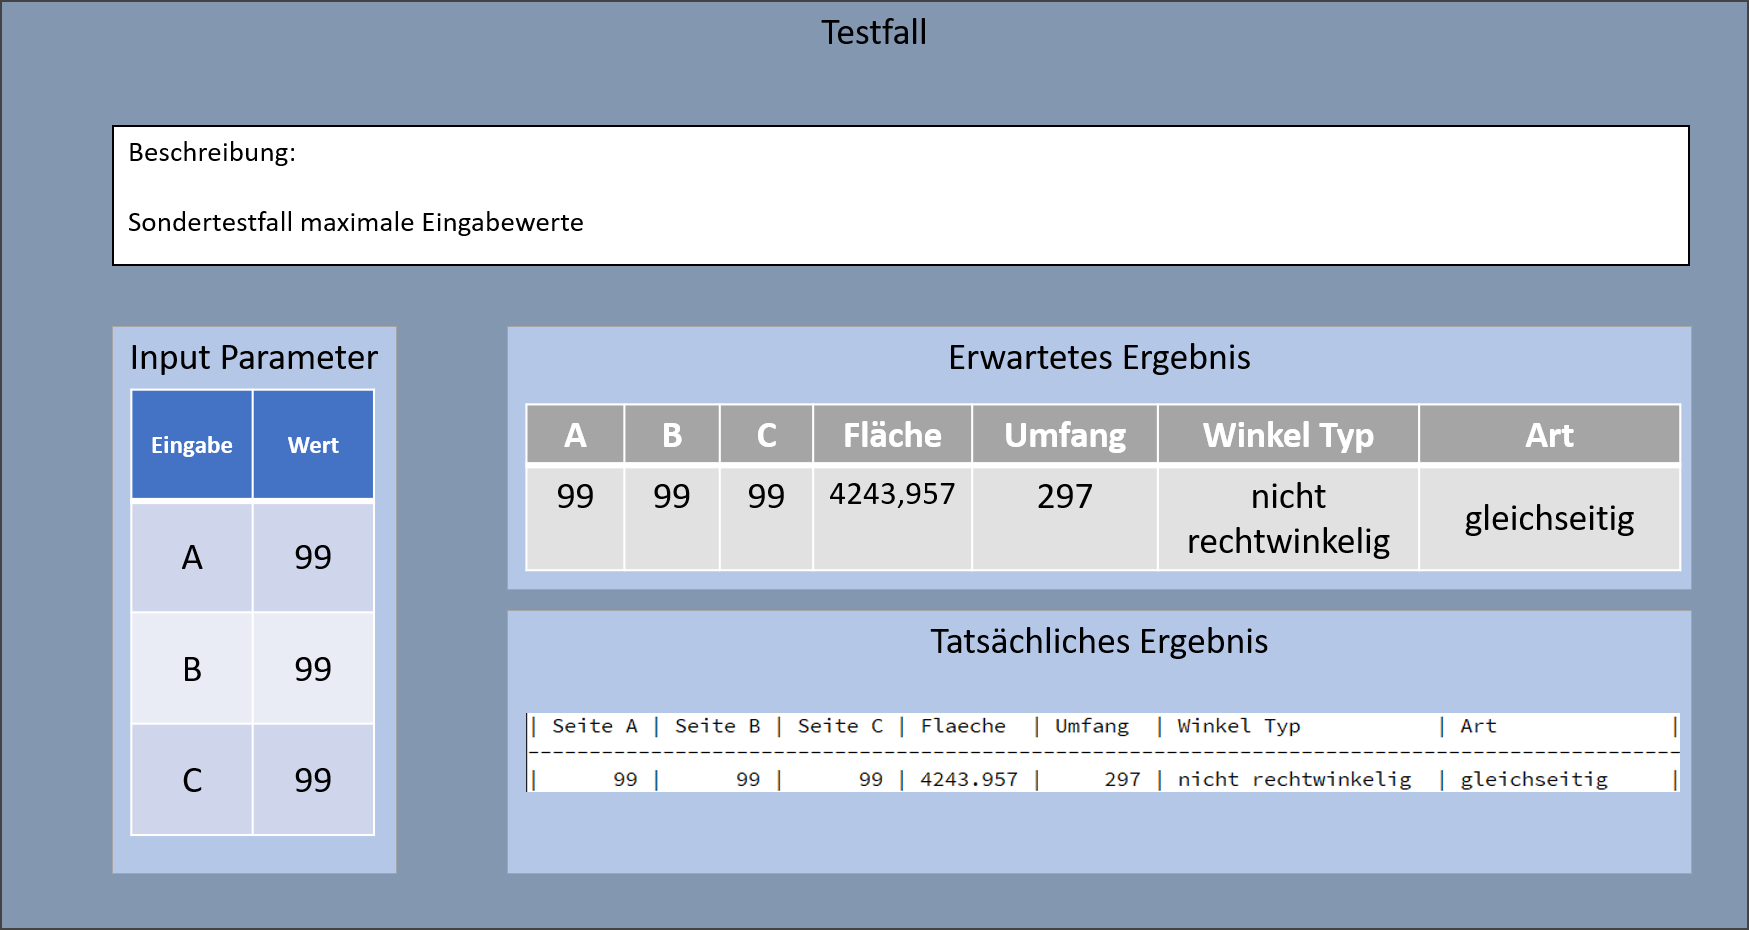
\includegraphics[width=\linewidth]{images/Testfall6.png}
    \caption{Testfall 6}
\end{figure}
\begin{figure}

    \centering
    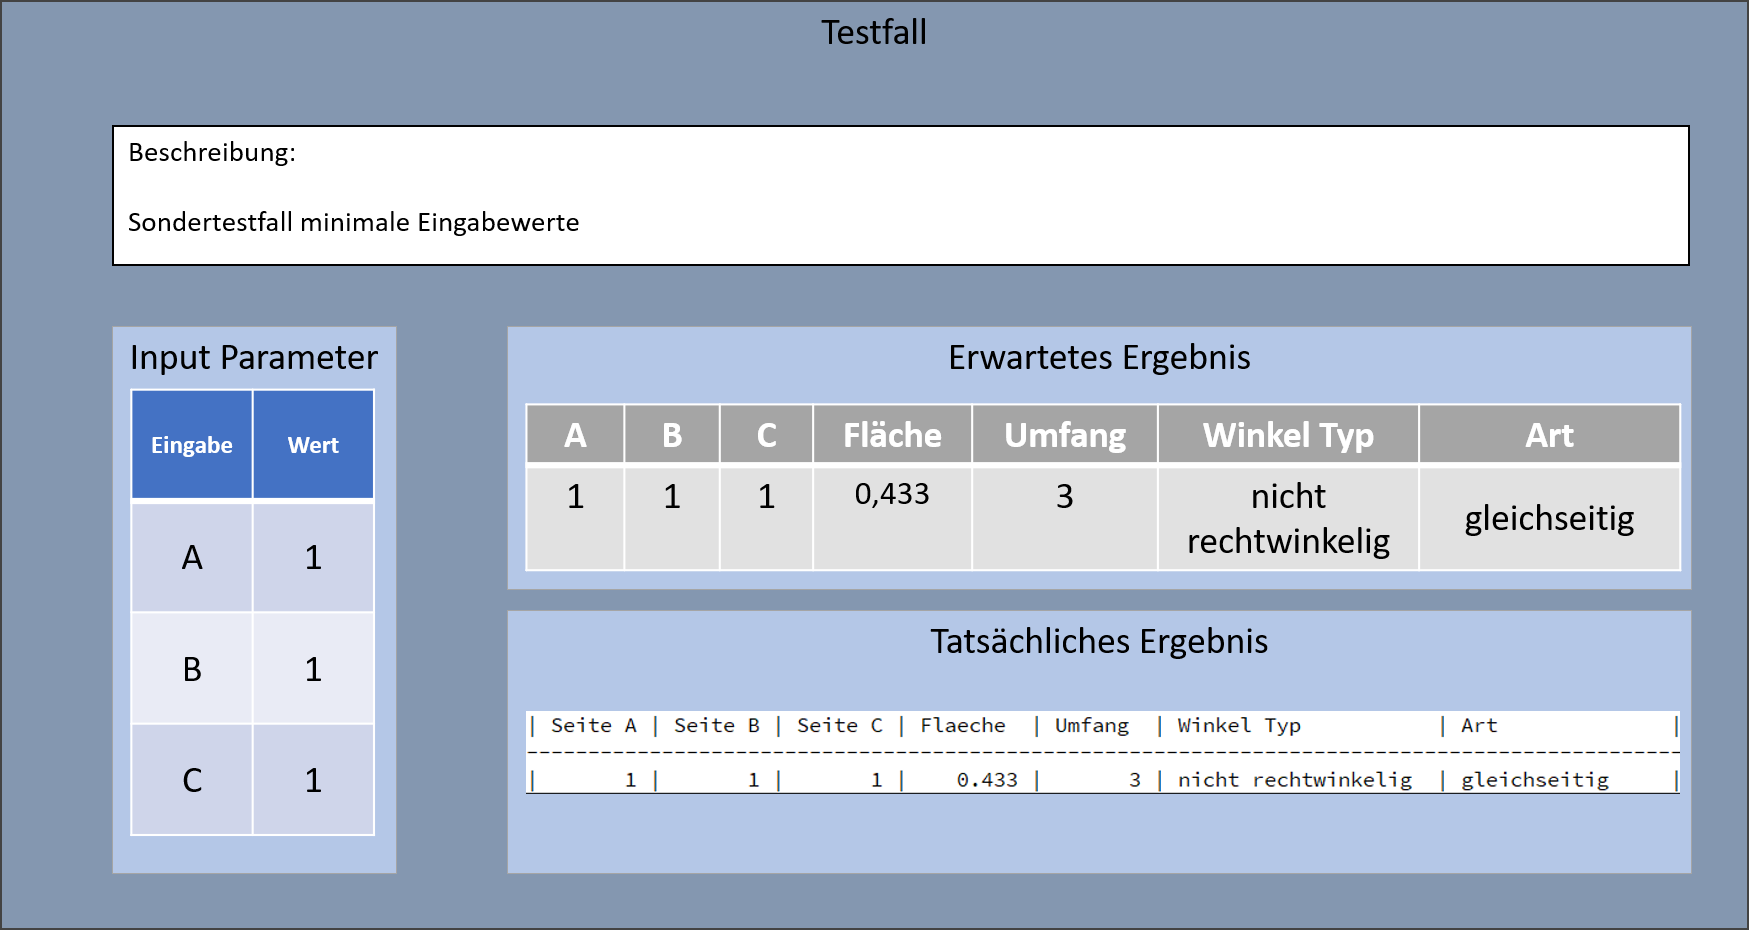
\includegraphics[width=\linewidth]{images/Testfall7.png}
    \caption{Testfall 7}
\end{figure}
    \addtocontents{toc}{\protect\newpage}
    % ============= Buchstabenteil ==============
    \renewcommand{\thechapter}{\Alph{chapter}}%
    \setcounter{chapter}{0}
    \chapter{Benutzeranleitung}\label{ch:benutzeranleitung}


\section{Vorbereiten des Systems}\label{sec:vorbereiten-des-systems}

\subsection{Systemvoraussetzungen}\label{subsec:systemvoraussetzungen}
Um das Programm zu benutzen ist ein Windows- oder Linux-System vorausgesetzt.
Unter Linux muss zusätzlich \textit{Wine}~installiert werden.

\subsection{Installation}\label{subsec:installation}
Die Installation des Programms erfolgt über das Entpacken der~.zip-Datei.
Die ausführbare .exe befindet sich im Anschluss im Unterordner \textit{bin}.
Außerdem ist es notwendig, dass unter Windows die PATH-Variable den Pfad zu GnuCOBOL/bin enthält.

\section{Programmaufruf}\label{sec:programmaufruf}
Um das Programm zu starten, muss die bin/TexteingabeHandy.exe aufgerufen werden.
Es öffnet sich ein Dialogfenster, mit welchem der Nutzer anschließend interagieren kann.


\section{Testen der Beispiele}\label{sec:testen-der-beispiele}
Die Beispiele können alle mittels der~.cmd-Dateien im bin Verzeichnis getestet werden.
Die TestAll.cmd enthält dabei alle Testfälle, welche automatisch nacheinander ausgeführt werden.
Hilfreich ist es, die ScreenBuffer-Size der Eingabeaufforderung auf eine höhere Zahl zu setzen, damit alle Zeilen in dem Dialogfenster bestehen bleiben.
Zu empfehlen ist hierbei eine Zahl über 1000.
    \chapter{Entwicklungsumgebung}\label{ch:entwicklungsumgebung}

Das Programm wurde mithilfe der OpenCobolIDE (\url{https://launchpad.net/cobcide/+download}) in der Version 4.7.6 geschrieben.
Dabei handelt es sich um eine leichtgewichtige COBOL Entwicklungsumgebung, die als Compiler GnuCOBOL 2.0.0 (\url{https://sourceforge.net/projects/gnucobol/}) verwendet.

Im Entwicklungsprozess wurde zur Versionsverwaltung GitHub (\url{https://github.com/}) verwendet.
Die dort angebotenen Remote-Repositories ermöglichen eine Versionierung und Backups des Quellcodes.

Alle Entwicklungsschritte wurden auf Systemen mit Windows 10 Betriebssystem (\url{https://www.microsoft.com/de-de/software-download/windows10}) durchgeführt.

\begin{figure}[htb]
    \centering
    \begin{minipage}{.5\textwidth}
        \centering
        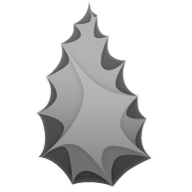
\includegraphics[width=.4\linewidth]{images/opencobol-logo}
    \end{minipage}%
    \begin{minipage}{.5\textwidth}
        \centering
        
\includegraphics[width=.4\linewidth]{images/Gnu-COBOL}
    \end{minipage}
    \caption{Logos von OpenCobolIDE und GnuCOBOL.}
    \label{fig:cobol-logos}
\end{figure}

\begin{figure}[htb]
    \centering
    
\includegraphics[width=.15\linewidth]{images/GitHub-Logo}
    \caption{
        GitHub-Logo.
    }
    \label{fig:github}
\end{figure}

    \chapter{Verwendete Hilfsmittel}\label{ch:verwendete-hilfsmittel}

Als Hilfsmittel wurden hauptsächlich die Inhalte der, von Prof. Dr. rer. nat. Karola Merkel (\url{https://www.fh-aachen.de/fachbereiche/medizintechnik-und-technomathematik/einrichtungen/sp-studienort-koeln/kontakt}) angebotenen, Vorlesung \glqq COBOL\grqq{} verwendet.
Zudem konnten unterschiedliche Fragen durch das Durchsuchen von Foren gelöst werden.
Besonders häufig konnte das \glqq Expertforum \glqq stackoverflow\grqq{} (\url{stackoverflow.com}) Antworten liefern.
    \chapter{Erklärung}\label{ch:erklaerung}

Hiermit versichere ich, dass ich die vorliegende Arbeit mit dem Thema
\begin{quote}
    \textit{\titleDocument}
\end{quote}
selbstständig verfasst und keine anderen als die angegebenen Quellen und Hilfsmittel benutzt habe.
Alle Ausführungen, die anderen Schriften wörtlich oder sinngemäß entnommen wurden, sind kenntlich gemacht und die Arbeit ist in gleicher oder ähnlicher Fassung noch nicht Bestandteil einer Studien- oder Prüfungsleistung.
\\

\vspace*{2cm}

\begingroup
\setlength{\parindent}{0pt} % keine Einrückung bei neuen Absätzen in diesem Bereich

\locationDocument, den \dateDocument
\bigskip
\bigskip

% gewünschte Breite der Unterschriftslinie
\newlength{\widthbox}
\settowidth{\widthbox}{\locationDocument, den \dateDocument}

\makebox[\widthbox]{\hrulefill}\\
\authorDocument
\endgroup
\newpage

    \chapter{Aufgabenstellung}\label{ch:aufgabenstellung}

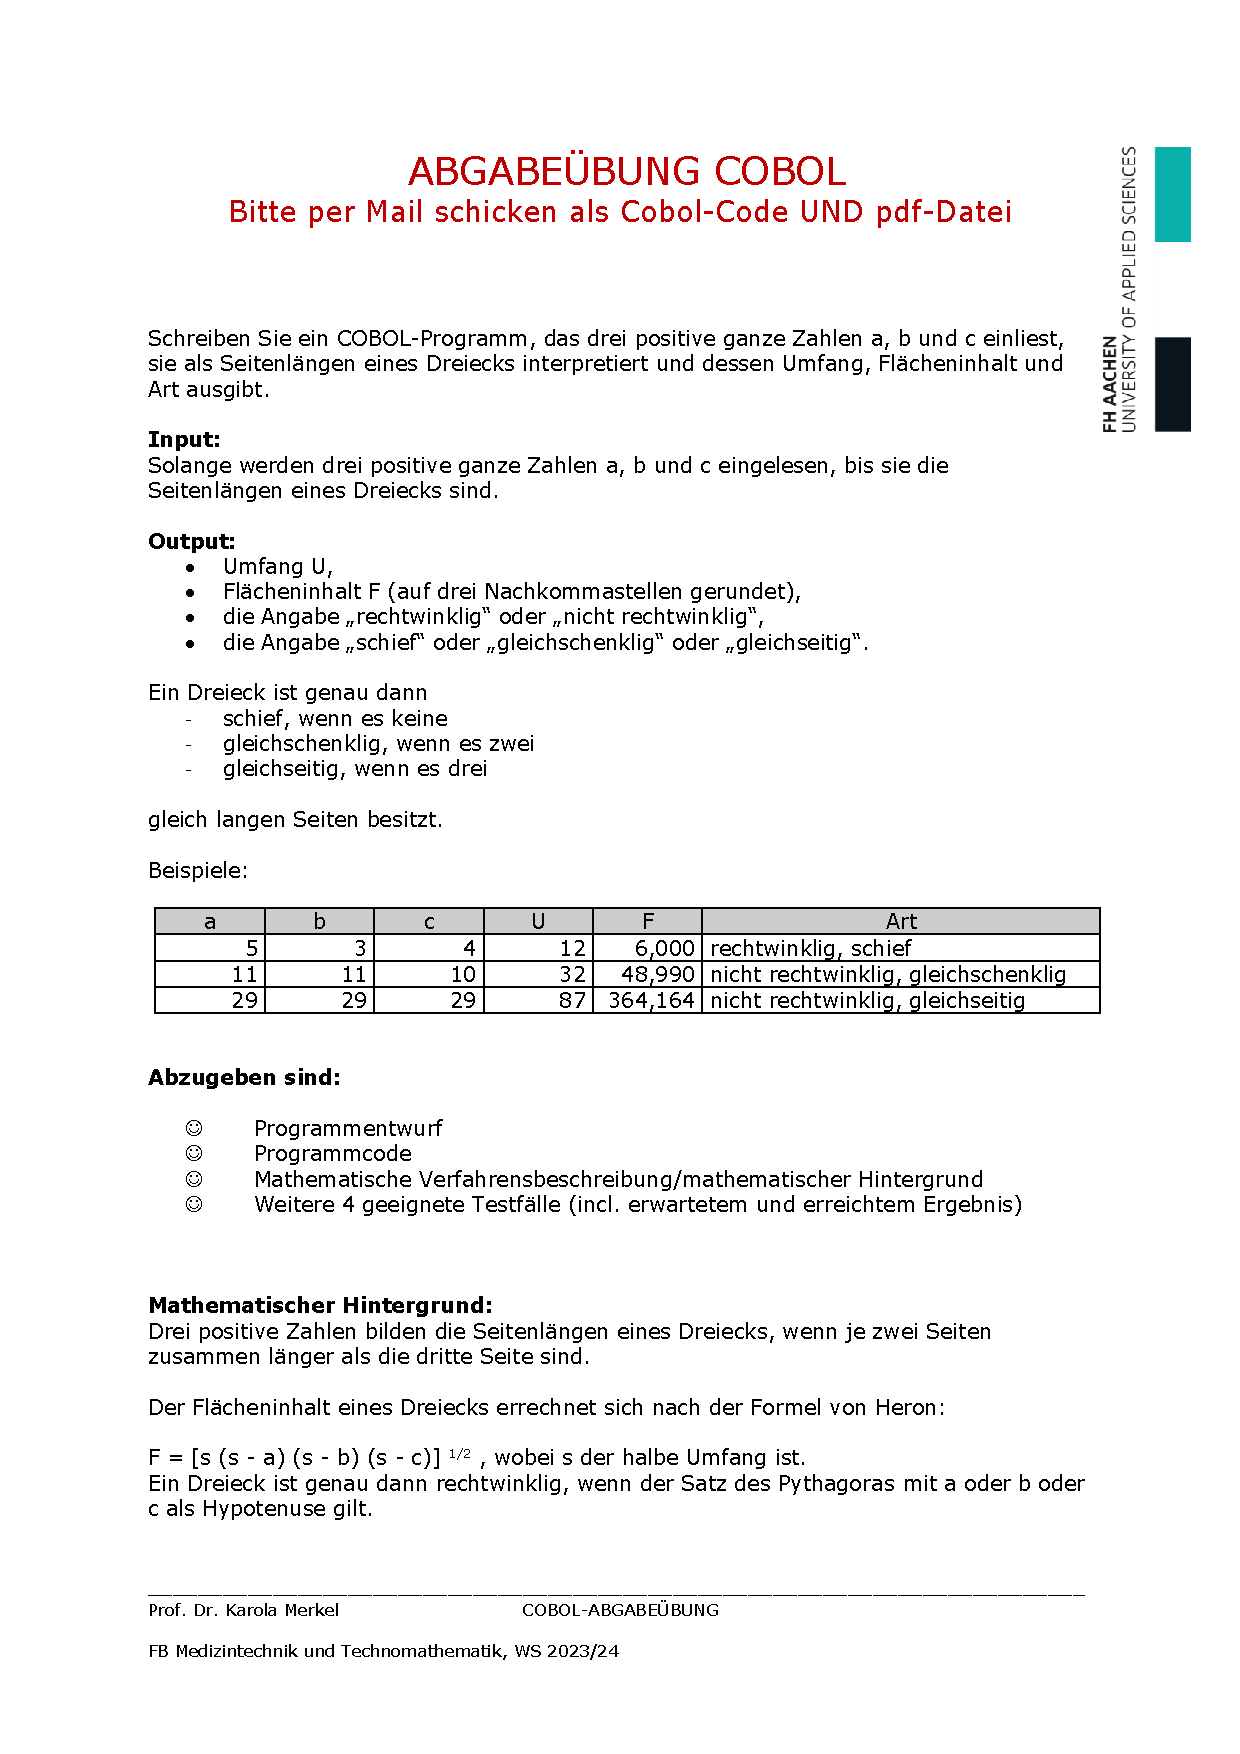
\includepdf[pages=-]{images/ABGABEUEBUNG 2023_23.pdf}
    \chapter{Quellcode}\label{ch:quellcode}
\end{document}
